\section{Moment information depends on the direction of the move}
\label{sec:directional-information}
The fourth- and eighth-return-moment assumptions used by the implementations
are sufficient for particular score constructions. They are not minimal
assumptions for all utility inference. Even a costless fixed-policy comparison shows a directional
asymmetry: ENTRY utility is bounded above, whereas cash-PARK utility gain is
bounded below. This section concerns explicit iid moment classes; the fixed
Laplace financial DGP imposes additional restrictions.

\subsection{An exact ENTRY frontier with a second-return-moment cap}
Fix $\gamma>0$ and a known $K_2>0$. Let $\mathcal P(K_2)$ contain all iid laws
of a fixed policy return $r$ with $\E r^2\le K_2$. The entry score against
cash is $U(r)=r-\gamma r^2/2$. Its null is
$\mathcal H_0=\{Q\in\mathcal P(K_2):\E_Q U(r)\le0\}$.
The tester may use the entire return sequence and independent randomization.

\begin{theorem}[A second-return-moment frontier for uniform ENTRY testing]
\label{thm:entry-frontier}
Let $\tau$ satisfy
$\sup_{Q\in\mathcal H_0}Q(\tau<\infty)\le\alpha$. For any
$P\in\mathcal P(K_2)$ with $\mu=\E_P r\le\gamma K_2/2$,
\begin{equation}
 P(\tau<\infty)\le\alpha,
 \label{eq:entry-impossible-region}
\end{equation}
including when $\E_P U(r)>0$. Conversely, there is a single valid test,
using only $K_2$ and $\gamma$, with eventual power one under every iid
$P\in\mathcal P(K_2)$ satisfying $\mu>\gamma K_2/2$.
The impossibility persists if all laws are restricted to have all absolute
moments finite, without common higher-moment bounds.
\end{theorem}
\begin{proof}
Put $m_2=\E_P r^2$. For $0<\varepsilon<1$, define the iid mixture
\begin{equation}
 a_\varepsilon=-\sqrt{\frac{K_2-(1-\varepsilon)m_2}{\varepsilon}},\qquad
 Q_\varepsilon=(1-\varepsilon)P+\varepsilon\delta_{a_\varepsilon}.
 \label{eq:entry-contamination}
\end{equation}
Its second moment is exactly $K_2$, and
\[
 \E_{Q_\varepsilon}U(r)
 =(1-\varepsilon)\mu
 -\sqrt{\varepsilon\{K_2-(1-\varepsilon)m_2\}}-\gamma K_2/2<0
\]
when $\mu\le\gamma K_2/2$. Coupling the mixtures bounds the total variation
distance between the first $n$ return histories by $n\varepsilon$. Therefore
$P(\tau\le n)\le\alpha+n\varepsilon$. First let $\varepsilon\downarrow0$
at fixed $n$, then $n\to\infty$, proving \eqref{eq:entry-impossible-region}.
Finite higher moments are preserved by each finite-point mixture.

For the converse, use the conservative statistic
\begin{equation}
 Z=r-\gamma K_2/2,\qquad
 \E Z\le\E U(r),\qquad
 \E Z^2\le(\sqrt{K_2}+\gamma K_2/2)^2=:\nu_Z^2.
 \label{eq:entry-surrogate}
\end{equation}
The original null implies $\E Z\le0$, so T1 applied to $Z$ with its public
bound is valid. Under the stated iid alternative, $Z$ has constant positive
mean. T2's capped past-mean bet, initialized with gain $\nu_Z/2$, gives crossing probability tending to
one. The bet uses no alternative-specific mean, proving the assertion.
\end{proof}

This specializes the total-variation null-density argument in
\cite[Section~2, Corollary~1]{impossible}. The proof first controls each finite
prefix, then sends the horizon to infinity; it requires no continuity of the
test. It is not a new general testing-impossibility principle.
It identifies the exact testable region for this utility and information
contract. For $\gamma=K_2=1$, deterministic return $r=.2$ has utility $.18$
but lies in the impossible region. A law's moments may be estimable from an
infinite iid sequence while finite-error sequential certification remains
impossible uniformly over the class. If $\gamma\sqrt{K_2}\ge2$, the testable
region is empty because $\mu\le\sqrt{K_2}$.
\begin{figure}[H]\centering
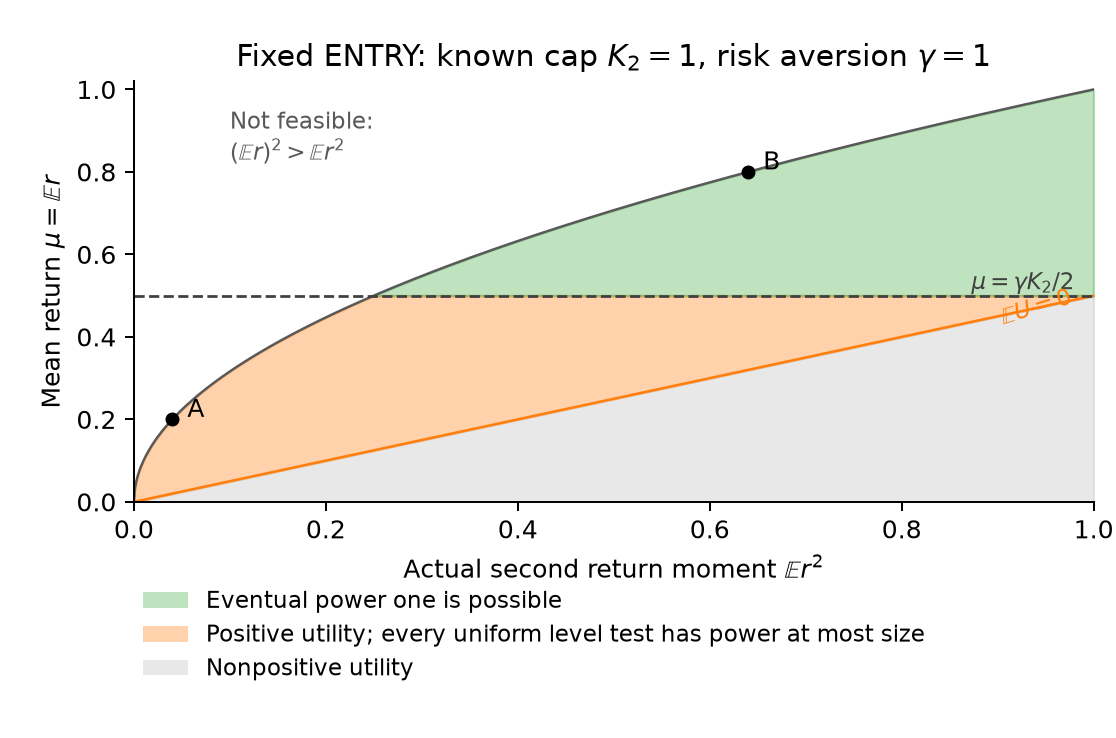
\includegraphics[width=.90\linewidth]{figures/directional_frontier.png}
\caption{Analytic regions for the fixed-policy iid moment class, not simulated
data. Feasibility requires $\mu^2\le\E r^2\le K_2$; positive utility requires
$\mu>\gamma\E r^2/2$. Uniformly informative ENTRY testing with only the public
cap requires the stronger $\mu>\gamma K_2/2$; its boundary belongs to the
impossibility region. Point A is deterministic return $.2$ with utility $.18$;
point B is deterministic return $.8$ with utility $.48$. Both are profitable,
but only B lies above this moment-class testing frontier.}
\label{fig:directional-frontier}
\end{figure}

For a positive-utility law in the impossible region, $m_2<K_2$. If
$m_4=\E_P r^4<\infty$, the contaminating null has
\[
 \E_{Q_\varepsilon}r^4=(1-\varepsilon)m_4
      +\frac{\{K_2-(1-\varepsilon)m_2\}^2}{\varepsilon}\longrightarrow\infty.
\]
Thus a valid numerical higher-moment envelope can rule out these nulls.
The second-return-moment surrogate is not merely inefficient in this region:
no uniformly valid test of the same class has nontrivial power there.
Joint conditional mean/variance tests are established \cite{meanvariance}.
On the iid class here, our null implies $\E r\le\gamma K_2/2$ and
$\operatorname{Var}r\le K_2$. These define a larger null that also contains
profitable laws below the frontier. A return-moment test for those bounds is
therefore conservative for our utility null; the targets are not equivalent.

\subsection{Moments strictly above two can suffice}
\begin{proposition}[A sufficient higher-moment route]
\label{prop:above-two}
Consider the iid class with a known $M<\infty$ bounding $\E|r|^{2+\xi}$
for some $\xi>0$.
Set $p=1+\xi/2$. A fixed countable mixture of bias-corrected lower-clipped
utility betting products is valid for $\E U(r)\le0$ and has eventual power
one at every iid positive-utility law obeying the bound.
\end{proposition}
Minkowski and Lyapunov give the required utility moment envelope
\begin{equation}
 \E|U(r)|^p\le
 \left\{M^{1/(2p)}+\frac\gamma2M^{1/p}\right\}^p=:A_p.
 \label{eq:utility-moment-conversion}
\end{equation}
Appendix~\ref{app:directional} gives the complete construction and proof.
This existence result uses a countable grid of clipping levels and small
stakes, rather than the finite nine-component financial rule. It asserts no
uniform delay or expected-time bound. Fourth/eighth moments are convenient
sufficient choices for the reported implementations, not minimal moment orders.

\subsection{Cash-PARK uses an economic lower bound}
Let $U(r)=r-\gamma r^2/2$, and compare cash with a predictable target
$w_t\in[-L,L]$ in a scalar return $A_t$, with $c=\eta=0$. The gain is
\begin{equation}
 Y_t=-w_tA_t+\frac\gamma2w_t^2A_t^2
     =\frac\gamma2(w_tA_t-\gamma^{-1})^2-\frac1{2\gamma}.
 \label{eq:cash-score}
\end{equation}
Consequently the ordinary linear betting process
\begin{equation}
 G_n=\prod_{t=1}^n(1+\gamma Y_t/2)
 \label{eq:cash-linear}
\end{equation}
has factors at least $3/4$. Under every law with finite conditional score
expectations and $\E_{t-1}Y_t\le0$, it is a test supermartingale, requiring
no supplied numerical fourth/eighth-return-moment cap. For iid scores with
$\E|Y_t|<\infty$ and $\E Y_t>0$, a fixed mixture over
$\lambda_j=\gamma2^{-j-1}$, weights $2^{-j-1}$, $j\ge0$, has eventual power
one; Appendix~\ref{app:directional} proves this with the small-stake argument.
The single stake $\gamma/2$ need not have this universal consistency.

These are specializations of standard safe linear betting and mixtures
\cite{savi,boundedbet}. The lower bound concerns cash versus this reference;
arbitrary reoptimized ENTRY, single-signal deletion and swap scores need not
have it. No new financial arm is substituted. The next section treats the
dependent scores of an estimated reference and the particular fixed capital
\eqref{eq:cash-linear}.
